%%%%%%%%%%%%%%%%%%%%%%%%%%%%%%%%%%%%%%%%%%%%%%%%%%%%%%
% A template for Wiley article submissions.
% Developed by Overleaf. 
%
% Please note that whilst this template provides a 
% preview of the typeset manuscript for submission, it 
% will not necessarily be the final publication layout.
%
% Usage notes:
% The "blind" option will make anonymous all author, affiliation, correspondence and funding information.
% Use "num-refs" option for numerical citation and references style.
% Use "alpha-refs" option for author-year citation and references style.

% MRM style
\documentclass[num-refs]{wiley-article}
% \documentclass[blind,num-refs]{wiley-article}

% simple style
% \documentclass[num-refs]{mrm2plain}

% added for highlighting
\usepackage{soul}

% added for nice links
\usepackage[breaklinks]{hyperref}

% added for margin notes
\usepackage{marginnote}

\bibliographystyle{vancouver-authoryear}

% Graphics. Always show the figures but float to the end
\usepackage[final]{subfig, listings}
\usepackage[nofiglist]{endfloat}

\graphicspath{{./figures/}}

\papertype{Full paper}

\title{Adaptive Baseline Fitting for $^{\textbf{1}}$H MR Spectroscopy Analysis}

% Use the \authfn to add symbols for additional footnotes and present addresses, if any. Usually start with 1 for notes about author contributions; then continuing with 2 etc if any author has a different present address.
\author[1]{Martin Wilson}

%\contrib[\authfn{1}]{Equally contributing authors.}

% Include full affiliation details for all authors
\affil[1]{Centre for Human Brain Health and School of Psychology, University of Birmingham, Birmingham, UK.}

\corraddress{Martin Wilson, Centre for Human Brain Health, University of Birmingham, Edgbaston, Birmingham, B15 2TT, United Kingdom.}

\corremail{wilsonmp@bham.ac.uk}

% Include the name of the author that should appear in the running header
\runningauthor{Wilson}

% my macros
\newcommand{\proton}{\ensuremath{^1\mathrm{H}}}
\newcommand{\bzero}{\ensuremath{\mathrm{B}_0}}
\soulregister\bzero7 % needed for soul to work with this macro
\soulregister\ref7 % needed for soul to work with this macro
\soulregister\cite7 % needed for soul to work with this macro

% revision one highlighting
\newcommand{\revone}[2]{\hl{#1}\marginnote{\hl{#2}}}
\newcommand{\revonenm}[1]{\hl{#1}} % no margin label

% uncomment next two lines to hide revision two highlighting
%\newcommand{\revone}[2]{#1}
%\newcommand{\revonenm}[1]{#1}

\begin{document}

\maketitle

\begin{abstract}
  \textbf{Purpose:} Accurate baseline modeling is essential for reliable MRS analysis and interpretation --- particularly at short echo-times, where enhanced metabolite information coincides with elevated baseline interference. The degree of baseline smoothness is a key analysis parameter for metabolite estimation, and in this study a new method is presented to estimate its optimal value. \\
  \textbf{Methods:} An adaptive baseline fitting algorithm (ABfit) is described, incorporating a spline basis into a frequency-domain analysis model, with a penalty parameter to enforce baseline smoothness. A series of candidate analyses are performed over a range of smoothness penalties, as part of a four stage algorithm, and the Akaike information criterion is used to estimate the appropriate penalty. ABfit is applied to a set of simulated spectra with differing baseline features and an experimentally acquired 2D MRSI dataset. \\
  \textbf{Results:} Simulated analyses demonstrate metabolite errors result from two main sources: bias from an inflexible baseline (underfitting) and increased variance from an overly flexible baseline (overfitting). In the case of an ideal flat baseline ABfit is shown to correctly estimate a highly rigid baseline, and for more realistic spectra a reasonable compromise between bias and variance is found. Analysis of experimentally acquired data demonstrates good agreement with known correlations between metabolite ratios and the contributing volumes of gray and white matter tissue. \\
  \textbf{Conclusion:} ABfit has been shown to perform accurate baseline estimation and is suitable for fully-automated routine MRS analysis.
  \keywords{ABfit; MRSI; spectral analysis; automated; open-source; spline}
\end{abstract}

Word count : 5535

% MRM abstract max length is 250 words (passive voice)
% MRM full paper max length is 5000 words, 10 fig plus tables

\section{Introduction}
A number of key metabolites may be detected using \proton\ Magnetic Resonance Spectroscopy (MRS), providing a non-invasive measure of healthy and diseased brain tissue metabolism. Clinical applications include the assessment of brain tumors, metabolic disorders and neonatal encephalopathy~\cite{Oz2014,Lally2019} where the concentration of certain metabolites may inform disease diagnosis or predict patient outcome. Further applications are present in the neuroscience and psychiatry domains, with particular interest in the direct detection of neurotransmitter levels such as GABA and glutamate --- which have been shown to be abnormal in Schizophrenia~\cite{Merritt2016} and modulate in response to tasks~\cite{Jelen2018,Chen2017}.

MRS scans are typically performed at short (30 ms) or long (144 ms) TE's, with short-TE scans being preferred due to reduced T2 relaxation and dephasing of multiplets resulting in improved metabolite detection sensitivity~\cite{Wilson2019}. However, short-TE scans are typically more susceptible to artefacts originating from insufficient water and scalp lipid suppression, in addition, broad signals from macromolecules also become enhanced~\cite{Cudalbu2012}. Residual water signals, lipid signals and macromolecules all have the potential to bias metabolite measurements due to spectral overlap and interference. Therefore, appropriate analysis methodology is particularly important to achieve the full benefit of MRS at short-TE.

Parametric fitting is currently the most widely used analysis method, and typically incorporates a set of simulated metabolite signals --- known as a basis set. \revone{An important distinction}{R0.1} between analysis methods is their approach for mitigating metabolite estimation bias from broad signals not present in the basis set, usually referred to as ``baseline modeling''. One of the most popular baseline modeling methods incorporates a set of smooth spline functions into the fitting procedure, with additional smoothness imposed by penalizing greater baseline complexity. The LCModel~\cite{Provencher1993} and AQSES~\cite{Poullet2007} algorithms both use penalized spline baseline modeling, with analysis performed in the frequency-domain and time-domain respectively.

An alternative approach to baseline modeling exploits the rapid decay of baseline signals in the time-domain by omitting the preliminary data points during the fitting process, reducing their interference with the more slowly decaying metabolites. The QUEST~\cite{Ratiney2005} and TARQUIN~\cite{Wilson2011} methods both use this time-domain truncation approach. The FITT~\cite{Young1998} algorithm combines the wavelet transform with Lowess filtering in the frequency-domain to separate metabolite and baseline signals.

Control over the level of baseline flexibility (or smoothness) is a common and necessary requirement of each of the baseline modeling methods outlined above. In spline based approaches, a combination of the number of spline functions for a given frequency range and the smoothness penalty parameter control the baseline flexibility. For LCModel, the frequency spacing between the spline basis functions is dependent on data quality, and is set at maximum of 1.5 times the estimated full width at half maximum (FWHM) of the metabolite resonances or 0.1 ppm~\cite{Provencher1993}. Similarly, for the FITT algorithm a fixed Lowess filter smoothing value is used and wavelet coefficients with scales less than twice the FWHM are excluded from the baseline model to ensure smoothness~\cite{Young1998}. In the time-domain truncation approach baseline flexibility is primarily determined by the number of initial data points to be omitted from the fit evaluation. For QUEST and TARQUIN the number of truncated data points, and therefore degree of baseline flexibility, is set at a default value that may be adjusted by the user.

Automated methods to determine the correct degree of baseline flexibility are important for obtaining accurate metabolite levels independently of the analyst. Furthermore, the manual adjustment of baseline flexibility for each individual spectrum is impractical for MRSI studies --- where hundreds of spectra may be acquired in a single scan. Whilst LCModel provides automated adjustment of baseline flexibility, a growing number of analysts choose to manually override the default analysis settings by adjusting the spline spacing parameter (DKNTMN). The first reported use of this manual adjustment was to improve the modeling of macromolecular resonances in rat brain at 9.4 T~\cite{Pfeuffer1999}. More recently, this parameter has been adjusted to encourage flatter baselines~\cite{Deelchand2016,Terpstra2010,Marjanska2018}, suggesting the default LCModel baseline flexibility may not be optimal in some cases.

Finding the optimal degree of baseline flexibility is a crucial question in MRS analysis research, yet few studies have investigated this topic in detail. Using simulated data, Ratiney et al.\ demonstrated how the interference between metabolite and baseline signals was reduced by increasing the number of omitted data points, but this came at the cost of inflating errors due to noise~\cite{Ratiney2004}. More recently, Near et al.\ showed how the estimated baseline in LCModel can depend strongly on spectral SNR and metabolite FWHM, and that errors caused by baseline instability may dominate over errors from spectral noise in some cases~\cite{Near2013}. The influence of baseline flexibility has also been explored using experimentally acquired data, with a recent study demonstrating a 15\% difference in metabolite levels when comparing between a default and less flexible baseline model~\cite{Giapitzakis2019}. Baseline flexibility has also been shown to have a strong influence of the measurement of 2-hydroxyglutarate~\cite{Wenger2019}.

In this study, we introduce a new method to automatically determine the optimal degree of baseline flexibility for a frequency-domain spline based fitting algorithm. Firstly, background is given on the use of penalized splines for optimal data smoothing. A fully-automated fitting algorithm is presented, incorporating a novel method to automatically estimate the optimal level of baseline flexibility. Finally, the new method is validated with simulated and experimentally acquired MRSI data.

\section{Theory}
\subsection{Penalized spline smoothing}

Baseline signals have a characteristically smooth spectral appearance, and \revone{must be}{R1.5} accurately modeled to avoid biasing metabolite estimates. In good quality \proton\ MRS of brain tissue baseline signals have a low intensity, relative to the primary metabolite resonances, and are therefore challenging to estimate in the presence of noise. Estimating a smooth function from noisy data is known in statistics as ``scatterplot smoothing'', and a number of approaches have been developed~\cite{Ruppert2003}. In this section we briefly outline the method of penalized splines in the simpler context of scatterplot smoothing, before describing their use as part of an MRS fitting algorithm.

\begin{figure}
  \begin{center}
    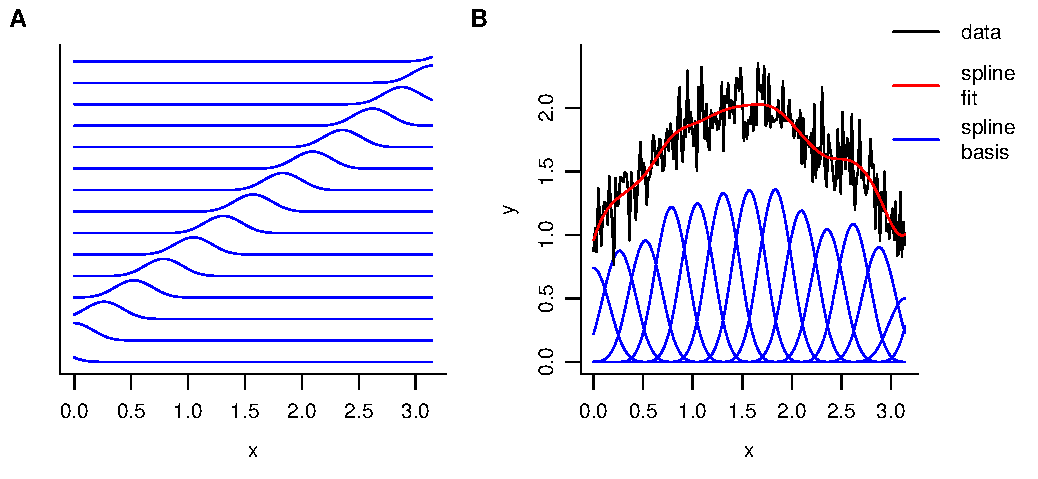
\includegraphics[width=1\textwidth]{fig1}
    \caption{A) Cubic B-spline basis of 15 components with each component offset vertically to reduce overlap. B) P-spline regression of a noisy signal with an underlying smooth trend.}
    \label{bspline_regression}
  \end{center}
\end{figure}

A spline is a piecewise function made up of one or more polynomial segments joined together at points known as ``knots''. A wide range of spline functions are possible, however Basis-splines, more commonly known as B-splines, are a popular choice for smoothing applications due to their favorable numerical properties~\cite{DeBoor2001}. The degree of a B-spline function determines its overall smoothness, and third degree (or cubic) B-splines are often used for smoothing. A cubic B-spline basis is show in Figure~\ref{bspline_regression}A with an offset added in the y-axis for clarity. B-spline bases consist of regularly spaced overlapping spline functions, spanning the full range of x values.

A B-spline basis may be used to obtain a smooth estimate of a signal using simple linear regression. Figure~\ref{bspline_regression}B shows the result of a spline regression, where each spline function has been optimally weighted, such that the sum of the functions (spline fit line) is the least squares fit to the data. The desired smoothness of the fit is controlled by adjusting the spline knot spacing, which in turn changes the density of spline functions. In the case of Figure~\ref{bspline_regression}B, 15 functions were found to give a reasonable level of smoothness. Increasing the density of spline functions allows more detail to be captured by the fit, however too many functions results in an increased sensitivity to noise and the smooth estimate begins to exhibit random fluctuations. Conversely, insufficient density of spline functions results in the spline fit being unable to model genuine smooth trends present in the data.

An alternative to adjusting the number of spline basis functions to achieve a desired level of smoothness is to introduce a penalty parameter into to spline regression model. The smooth estimate $\hat{\mathbf{y}}$, of our data $\mathbf{y}$, is calculated as: $\hat{\mathbf{y}} = \mathbf{B} \ \hat{\mathbf{a}}$, where $\mathbf{B}$ is a B-spline basis in matrix form, and $\hat{\mathbf{a}}$ is a vector of corresponding spline weightings to be determined. In simple spline regression $\hat{\mathbf{a}}$ is found by solving the normal equations to minimize the sum of the squared differences between $\mathbf{y}$ and $\hat{\mathbf{y}}$. In penalized spline regression, the minimization function $Q_B$ is adjusted to incorporate an additional term to enforce smoothness in the estimate:

\begin{equation}
  Q_{B} = \|\mathbf{y} - \mathbf{B} \ \hat{\mathbf{a}} \|^{2}_{2} + \lambda \|\mathbf{D} \ \hat{\mathbf{a}}\|^{2}_{2}.
  \label{qb}
\end{equation}

The $\lambda$ parameter controls the degree of smoothness by penalizing solutions for $\hat{\mathbf{a}}$ that interact with the difference matrix $\mathbf{D}$. The difference matrix may be constructed to penalize the first, second or higher orders of differences between $\hat{\mathbf{a}}$ values. Here, we exclusively use a second order difference matrix, which acts to minimize the second derivative of the smooth estimate.

\begin{equation}
  \mathbf{D} =
  \begin{bmatrix*}[r]
    1 & -2 &  1 &  0 &  0 &  0 & \dots \\
    0 &  1 & -2 &  1 &  0 &  0 & \dots \\
    0 &  0 &  1 & -2 &  1 &  0 & \dots \\
    0 &  0 &  0 &  1 & -2 &  1 & \dots \\
    \vdots & \vdots & \vdots & \vdots & \vdots & \vdots & \ddots \\
  \end{bmatrix*}
  \label{d_mat}
\end{equation}

An example of the second order difference matrix is given in~(\ref{d_mat}), which shows how increased differences between adjacent weighting factors in $\hat{\mathbf{a}}$ consequently increase the penalty term in Equation~(\ref{qb}). The minimization function $Q_{B}$ represents a compromise between minimizing the fit residual and smoothness, where a value of zero for $\lambda$ results in simple spline regression. Larger values of $\lambda$ encourage a smoother $\hat{\mathbf{y}}$, to the point where $\hat{\mathbf{y}}$ becomes a straight line fit for very large penalties when using a second order difference matrix. The solution to Equation~(\ref{qb}) may be found by augmenting $\mathbf{B}$ and $\mathbf{y}$:

\begin{equation}
  \begin{bmatrix}
    \mathbf{y} \\ 0
  \end{bmatrix}
  \approx
  \begin{bmatrix}
    \mathbf{B} \\ \sqrt{\lambda} \ \mathbf{D}
  \end{bmatrix} \hat{\mathbf{a}} =
  \begin{bmatrix}
    \hat{\mathbf{y}} \\ 0
  \end{bmatrix},
  \label{p-spline_eq}
\end{equation}

and regressing the augmented $\mathbf{y}$ vector on the augmented $\mathbf{B}$ matrix to yield $\hat{\mathbf{a}}$.

The general approach for penalized spline regression is to over-specify the number of B-spline basis functions, and primarily control the smoothness through the adjustment of $\lambda$ acting on a difference matrix. We refer to this approach as ``P-splines'', first introduced by Eilers and Marx~\cite{Eilers1996}. Whilst the value of $\lambda$ has a direct effect on smoothness, it is an unintuitive parameter to interpret, as the optimal value often varies by several orders of magnitude. In addition, $\lambda$ has a complex dependence on the density of the spline functions, the number of data points and other factors unrelated to smoothness. A more intuitive measure of the smoothness of a P-spline model is known as the effective dimension (ED), proposed by Hastie and Tibshirani \cite{Hastie1990}. For a given value of $\lambda$, B-spline basis $\mathbf{B}$ and difference matrix $\mathbf{D}$, we calculate ED as follows:

\begin{equation}
  \mathbf{H} =
  \begin{bmatrix}
    \mathbf{B} \\ \sqrt{\lambda}\ \mathbf{D}
  \end{bmatrix}^{-1}
  \begin{bmatrix}
    \mathbf{B} \\ 0
  \end{bmatrix},
\end{equation}

\begin{equation}
  \textsf{ED} = \textsf{tr}(\mathbf{H}),
\end{equation}

where $\textsf{tr}$ denotes the trace of a matrix. For a small value of $\lambda$, ED approaches the number of spline functions in the basis $\mathbf{B}$, and for large values, ED approaches 2 when using a second order difference matrix.

\begin{figure}
  \begin{center}
    \includegraphics[width=0.9\textwidth]{fig2}
    \caption{A) Penalized spline smoother applied to a simulated sine function over a range of smoothness penalties $\lambda$. B) Plots of the fit residual, smoother effective dimension (ED), fit error and Akaike information criterion (AIC) as a function of $\lambda$.}
    \label{pspline_error}
  \end{center}
\end{figure}

Using simulated data we investigate the relationship between $\lambda$, ED and the optimal level of smoothness. The top left panel in Figure \ref{pspline_error}A shows a simple sine function with added normally distributed noise, shown in red and black respectively. Candidate P-spline smoothers, with differing values of $\lambda$, are shown in the remaining 5 panels. Since the true shape of the underlying smooth function is known, the error of the P-spline estimate may be calculated as the sum of squared differences between the true function and the estimate. A plot of the error as a function of $\lambda$ is shown in Figure \ref{pspline_error}B. The sum of squared differences between the P-spline estimate and noisy data (residual) and the ED are also shown as a function of $\lambda$ in part B.

Inspection of the error plot reveals the optimal $\lambda$ to be approximately 20 --- corresponding to an ED value of 12, and this can be intuitively verified from part A. For larger values of $\lambda$, the estimate approaches a straight line fit --- failing to capture the details in the sine cure and resulting in an increasing fit residual and fit error (part B). Models with insufficient freedom to adapt to genuine trends in the data result in biased estimates and this is known as ``underfitting''. Conversely, too much freedom in the smoothing model (small $\lambda$) results in the estimate becoming overly sensitive to random fluctuations in the data resulting in ``overfitting''. In least-squares fitting, there is a temptation to equate the smallest residual with the optimal fit, however Figure \ref{pspline_error}B clearly shows an increase in the error for $\lambda$ values of less than 20 --- despite a steady reduction in the residual.

Determining the optimal value for the smoothness parameter is one of the primary challenges for P-spline smoothing. A careful balance between instability from overfitting, and bias from underfitting, must be made for the most accurate estimate, and searching for the smallest fit residual is a useful, but insufficient metric of quality. Numerous approaches have been proposed to find the optimal smoothing value \cite{Ruppert2003}, and in this study we use \textit{Akaike's information criterion} (AIC) \cite{Akaike1973}:

\begin{equation}
  \textsf{AIC} = \ln \left[ \|\mathbf{y} - \hat{\mathbf{y}}\|^{2}_{2} \right] + 2 \textsf{ED} / n,
  \label{aic}
\end{equation}

where $\ln$ denotes the natural logarithm and $n$ is the number of data points. The AIC is typically used to compare models, with lower values indicating an improved balance between bias and instability. A plot of the AIC as a function of $\lambda$ is shown in the lower panel of Figure \ref{pspline_error}B, and the $\lambda$ value with the lowest AIC shows good agreement with the true minimum error.

\subsection{MRS baseline estimation using P-splines}

In $^1\mathrm{H}$ MRS analysis, the baseline signal must be estimated in the presence of numerous overlapping metabolite lipid and macromolecule signals. Fortunately, these non-baseline signals have a known molecular origin and are therefore well characterized and accurately simulated from established parameters \cite{Govind2015}. We can update Equation \ref{p-spline_eq} to incorporate these additional molecular components by arranging into columns of the basis matrix $\mathbf{M}$, and appending to the P-spline basis $\mathbf{B}$:

\begin{equation}
  \begin{bmatrix}
    \textbf{y} \\ 0
  \end{bmatrix}
  \approx
  \begin{bmatrix}
    \textbf{B} && \textbf{M} \\ \sqrt{\lambda} \ \textbf{D} && 0
  \end{bmatrix} \hat{\mathbf{a}} =
  \begin{bmatrix}
    \hat{\textbf{y}} \\ 0
  \end{bmatrix},
  \label{mrs_bl}
\end{equation}

As with Equation \ref{p-spline_eq}, we regress the basis matrix on $\mathbf{y}$ to yield $\hat{\mathbf{a}}$, however since metabolite signal amplitudes are always positive, analysis stability may be improved by enforcing a non-negative constraint on the subset of $\hat{\mathbf{a}}$ values corresponding to the weightings on the molecular basis ($\hat{\mathbf{a}}_{M} \geq 0$). The active-set method developed by Lawson and Hanson \cite{Lawson1995} is used herein to find the least-squares solution under the non-negative constraint --- while still allowing the $\hat{\mathbf{a}}$ values corresponding to the spline basis ($\hat{\mathbf{a}}_{B}$) to remain unconstrained.

A simulation study was performed to investigate the relationship between baseline smoothness, the accuracy of metabolite estimates and the AIC. Metabolite signals were simulated from known parameters \cite{Govind2015} at levels consistent with normal brain tissue \cite{deGraaf2018} --- listed in Supporting Information Table S1. An experimentally derived macromolecule profile was also included in the simulation and basis matrix to yield a realistic spectrum~\cite{Birch2017}. Simulated experimental conditions consisted of a field strength of 3 T, and semi-LASER localization (TE=28 ms). 1024 complex points were generated at a sampling frequency of 2000 Hz, 6 Hz Gaussian line-broadening was applied prior to zero-filling to 2048 points and Fourier transform to the frequency-domain. Ideal pulses were assumed and relaxation effects were not considered.

Ideal spectra were distorted with normally distributed noise resulting in a spectral SNR of 54 --- with signal measured as the highest data point from the \revone{nominal NAA singlet peak}{R1.10} at 2.01 ppm. A broad Gaussian resonance was added at 1.3 ppm with a linewidth of 100 Hz to simulate baseline distortion originating from scalp lipids. The degree of P-spline baseline flexibility is defined as the baseline ED (effective dimension) per ppm, which is more easily compared across analyses due to its independence from the number of points in the fit and the number of spline basis functions used. Metabolite level estimates ($\hat{\mathbf{a}}$) were calculated using Equation \ref{mrs_bl} from real-valued data points in spectral region between 0.2 and 4 ppm, over a range of 10 levels of baseline flexibility. 32 spectra were generated at each level of baseline flexibility with differing noise samples drawn from the same distribution. The metabolite estimation error was calculated from the sum of the squared differences between the true and estimated values for each spectrum. The mean and standard deviation of metabolite estimation errors was calculated across the 32 spectra at each level of baseline flexibility to evaluate accuracy and consistency.

Metabolite estimation errors are shown in Figure \ref{mrs_bl_simple}A, displaying a comparable shape to the simpler model in Figure \ref{pspline_error}B. Over the range of baseline flexibility studied, underfitting with an inflexible baseline results in much greater metabolite estimate errors compared to overfitting --- which can be verified by inspecting the fit result plots in Figure \ref{mrs_bl_simple} parts C-F. Good agreement is also seen between the metabolite estimate error and the AIC curve (part B), with a low AIC values corresponding to the most accurate level of baseline flexibility.

From the results presented in following sections, it was found that the AIC had a tendency to slightly overestimate the optimal level of baseline flexibility, and that a simple modification to Equation \ref{aic} improved accuracy:

\begin{equation}
  \textsf{mAIC} = \ln \left[ \|\mathbf{y} - \hat{\mathbf{y}}\|^{2}_{2} \right] + 2 m \ \textsf{ED} / n.
  \label{maic}
\end{equation}

Setting $m$ to a value of 5 was found to be a good compromise between bias and variance, placing a greater penalty on overly flexible baseline models --- resulting in a smoother baseline estimate relative to the standard AIC (Figure \ref{mrs_bl_simple}B).

\begin{figure}
  \begin{center}
    \includegraphics[width=0.9\textwidth]{fig3}
    \caption{P-spline MRS baseline estimation of simulated data with a broad artefact at 1.3 ppm. A) metabolite estimate error as a function of baseline flexibility. Error bars represent standard deviations, increased by a factor of 5 to aid visualization. B) AIC and modified-AIC as a function of baseline flexibility. C) - F) Fit results with the baseline shown (black) underlying the simulated data (black) and fit (red). The fit residual is shown above the data and fit results are presented for the following values of baseline ED per ppm: C) 1, D) 4.2, E) 6.0, F) 25.}
    \label{mrs_bl_simple}
  \end{center}
\end{figure}

\section{Methods}
\subsection{Adaptive Baseline Fitting Algorithm}
In this section we describe a fully-automated $^1\mathrm{H}$ MRS analysis method based on the P-spline fitting approach presented in the Theory section. The emphasis of the design is to automatically adapt the baseline flexibility for improved accuracy, and we refer to the full algorithm as: \textit{Adaptive Baseline fitting} or ABfit. The algorithm consists of 4 main steps, which will be described in order of execution:

\begin{enumerate}
  \item Coarse frequency alignment.
  \item Approximate iterative fitting.
  \item Baseline smoothness estimation.
  \item Detailed iterative fitting.
\end{enumerate}

\subsubsection{Coarse frequency alignment (step 1)}
Unprocessed MRS data typically have an unknown and erroneous frequency offset $f_{o}$ that displaces all resonances equally. The first step of ABfit is to estimate $f_{o}$ (measured in Hz) to ensure the basis set of known signals are approximately matched to the acquired data. Raw MRS data is digitally sampled at a frequency of $\mathit{fs}$ Hz in the time-domain, and defined a vector of $N$ complex data points:

\begin{equation}
  \mathbf{y}^{\mathrm{TD}} = \mathbf{y}(\mathbf{t}), \mathbf{t}=(t_{1}=0,t_{2} =1/\mathit{fs},\ldots,t_{N}=(N-1)/\mathit{fs}),
\end{equation}

\begin{equation}
  \mathbf{y}^{\mathrm{FD}} = \mathbf{y}(\mathbf{f}), \mathbf{f}=(f_{1}=-\mathit{fs}/2,f_{2} =-\mathit{fs}/2 + \mathit{fs}/N ,\ldots,f_{N}=\mathit{fs}/2 - \mathit{fs}/N),
\end{equation}

where superscript TD and FD denote time and frequency-domain signal representations --- calculated with the discrete Fourier transform. We simulate a reference data set $\mathbf{r}^{\mathrm{TD}}$, with twice the number of data points $2N$ sampled at $\mathit{fs}$, containing three resonances corresponding to the main singlet metabolites typically present in $^1\mathrm{H}$ MRS data at 2.01, 3.03 and 3.22 ppm. The acquired data $\mathbf{y}^{\mathrm{TD}}$ is zero-filled to twice the original length --- before convolving with  $\mathbf{r}^{\mathrm{TD}}$ to estimate the frequency offset $f_{o}$ \revone{\cite{Provencher1993}}{R1.15}.

\subsubsection{Approximate iterative fitting (step 2)}
The goal of this stage of the algorithm is to find estimates of the three parameters with the largest influence on the fit residual: 1) the signal phase $\phi_{0}$; 2) an approximate lineshape parameter $d_{g}$ and 3) an improved estimate of $f_{o}$. The phase and frequency offset are applied to the acquired data as follows:

\begin{equation}
  \mathbf{y'}^{\mathrm{TD}} = \mathbf{y}^{\mathrm{TD}} e^{i \phi_{0} + 2 i \pi f_{o} \mathbf{t}}
\end{equation}

The lineshape parameter applies Gaussian line-broadening to each signal in the basis set $\mathbf{M}$, and the scaling factor $\beta$ is introduced to define $d_{g}$ as the Full Width at Half Maximum (FWHM) measured in Hz:

\begin{equation}
  \beta = -\frac{{(\pi d_{g} / 2)}^{2}}{\ln(1/2)},
  \revone{}{R1.16}
\end{equation}

\begin{equation}
  \mathbf{M}'^{\mathrm{TD}} = \mathbf{M}^{\mathrm{TD}} \star e^{-\beta \mathbf{t}^{2}},
\end{equation}

where $\star$ denotes element-wise multiplication of the line-broadening function for each column of the basis matrix. Combining the modified basis with the P-spline basis and solving for $\hat{\mathbf{a}}$ in the least-squares sense with the same constraints as the previous section:

\begin{equation}
  \begin{bmatrix}
    \textbf{y}'^{\mathrm{FD}}_{s} \\ 0
  \end{bmatrix}
  \approx
  \begin{bmatrix}
    \textbf{B} && \textbf{M}'^{\mathrm{FD}}_{s} \\ \sqrt{\lambda} \ \textbf{D} && 0
  \end{bmatrix} \hat{\mathbf{a}} =
  \begin{bmatrix}
    \hat{\textbf{y}} \\ 0
  \end{bmatrix}.
  \label{linear_fit}
\end{equation}

Note that following parametric modification in the time-domain, the data and basis of known signals are zero-filled to twice their original length before being transformed to the frequency-domain. Only the real valued data points in frequency domain between 1.8 and 4 ppm are fit in this stage of the algorithm (denoted by subscript $s$) to reduce the influence of any contaminating lipid signals around 1.3 ppm. The parameters: $\phi_{0}$, $d_{g}$ and $f_{o}$ are estimated using Nelder-Mead simplex algorithm with bound constraints \cite{Box1965}, minimizing:

\begin{equation}
  \| \textbf{y}'^{\mathrm{FD}}_{s}  - \hat{\textbf{y}} \|^{2}.
  \label{obj_fn}
\end{equation}

A $\lambda$ value corresponding to 1 ED per ppm is used with a P-spline basis with 15 components per ppm. Constraints are placed on the optimization algorithm to restrict the linebroading parameter to be positive and produce additional line-broadening of less than 15 Hz FWHM. The frequency offset is specified to be less than 10 Hz different from the coarse frequency alignment (step 1).

\subsubsection{Baseline smoothness estimation (step 3)}
Following the determination of the frequency offset, spectral phase and approximate lineshape the next step of ABfit is to estimate the optimal value for $\lambda$. A set of candidate fits are performed with differing level of baseline smoothness, whilst maintaining the three main fitting parameters constant at their optimized values. The maximum candidate baseline flexibility is set to a $\lambda$ value corresponding to 7 ED per ppm, and the minimum value set to an ED of 2 --- equivalent to straight line fit. 20 candidate fits are performed with logarithmic intervals between the maximum and minimum values, and the mAIC is calculated for each fit (Equation \ref{maic}). The optimal $\lambda$ value is found by selecting the candidate fit with the lowest mAIC. In contrast to the previous step, a wider spectral range of 0.2 to 4 ppm is analyzed to include the majority of conventionally measured metabolites.

\subsubsection{Detailed iterative fitting (step 4)}
In the final stage of ABfit, the overall lineshape model is refined alongside $f_{o}$, $\phi_{0}$ and minor adjustments to the frequencies and linewidths of the known basis signals. An asymmetric lineshape model is generated in the frequency-domain by smoothly adjusting the Gaussian linewidth parameter as a function of frequency --- as described by Stancik and Brauns~\cite{Stancik2008}:

\begin{equation}
  \mathbf{l}^{\mathrm{FD}} = \sqrt{\frac{4 \ln 2}{\pi}} \exp \left[ -4 \ln2 \left( \frac{\mathbf{f}}{\mathbf{s}(\mathbf{f})} \right) \right],
\end{equation}

\begin{equation}
  \mathbf{s}(\mathbf{f}) = \frac{2 d_{g}}{1 + \exp(a_{g} \ \mathbf{f})}.
\end{equation}

Note, the frequency dependence on the linewidth function is eliminated that when the asymmetry parameter $a_{g}=0$, leading to $\mathbf{s}=d_{g}$ and pure Gaussian broadening. $\mathbf{l}^{\mathrm{FD}}$ is transformed to the time-domain and applied to each of the molecular basis signals. Minor individual changes in the frequency offset and linewidth are applied to each molecular signal in the basis to accommodate variations in the acquired data:

\begin{equation}
  \mathbf{M}'^{\mathrm{TD}} = \mathbf{M}^{\mathrm{TD}} \star \mathbf{l}^{\mathrm{TD}} \star e^{(2i \pi \mathbf{f_{i}} - \pi \mathbf{d_{i}} ) \mathbf{t}},
\end{equation}

where $\mathbf{f_{i}}$ is a column vector of frequency adjustments measured in Hz, and $\mathbf{d_{i}}$ a column vector of additional Lorenzian line broadening terms measured at FWMH in Hz. Both parameter vectors $\mathbf{f_{i}}$ and $\mathbf{d_{i}}$ are the same length as the number of molecular basis signals. Each of the global ($f_{o}$, $\phi_{0}$, $d_{g}$, $a_{g}$) and molecular basis signal specific ($\mathbf{f_{i}}$, $\mathbf{d_{i}}$) parameters are estimated using the Levenberg–Marquardt algorithm \cite{Levenberg1944} implemented with bound constraints, with the same objective function defined in Equations \ref{linear_fit} and \ref{obj_fn}. The optimal baseline smoothness parameter $\lambda$, (determined in step 3) is used, and the spectral range of 0.2 to 4 ppm included in the iterative optimization procedure. The same parameter constraints were used as in step 2, with the additional lineshape asymmetry parameter $a_{g}$ being bound between $\pm$0.25, $\mathbf{f_{i}}$ bound between $\pm1$ Hz and  $2 \geq \mathbf{d_{i}} \geq 0$ Hz.

\subsection{Validation with simulated data}
A series of simulations were performed to evaluate the performance of ABfit across a range of common baseline features. For each test, ABfit was performed as described in the previous section --- where the baseline flexibility is automatically determined in step 3. Additionally, ABfit was performed with the baseline flexibility set manually (omitting step 3) across a range of 15 values for ED per ppm between 0.53 and 15 to compare with the automated result. Simulated spectra and metabolite estimation errors were calculated as described in section \textit{MRS baseline estimation using P-splines} unless stated otherwise.

In the first simulation study a broad simulated peak with a Gaussian lineshape (FWHM 100 Hz) at 1.3 ppm was combined with metabolites and the macromolecular signal with a spectral SNR of 54. The second simulation study was identical to the first, however the broad simulated peak was removed to yield a perfectly flat baseline. The third simulation study was identical to the first, however the amplitude of the simulated broad resonance was increased by a factor of 2. The data for the fourth simulation study was identical to the second, with a perfectly flat baseline and an experimentally derived macromolecular signal. However, the experimentally derived macromolecular signal was removed from the fitting basis set and replaced with the set of simulated lipid and macromolecular signals commonly used by default in the LCModel and TARQUIN algorithms, as listed in Supporting Information Table S2. The final simulation study was identical to the first, however 12 Hz linebroading was applied to the molecular basis rather than 6 Hz --- resulting in a spectral SNR of 34.

\subsection{Validation with experimentally acquired data}
%Whilst simulation studies are important to assess the true accuracy of a method, it is challenging to accurately reproduce the true range of variation present in MRS data. Therefore, ABfit was tested on experimentally acquired MRSI data to ensure validity and robustness to typical distortions such as residual water, shimming variations and minor shifts in metabolite frequency.

MR data was acquired from a healthy adult male with a 3 T Siemens Magnetom Prisma (Siemens Healthcare, Erlangen, Germany) system using a 32-channel receiver head coil-array. T1-weighted MRI was acquired with a 3D-MPRAGE sequence: FOV = 208 x 256 x 256 mm, resolution = 1 x 1 x 1 mm, TE/TR = 2 ms/2000 ms, inversion time = 880 ms, flip angle = 8 degrees and GRAPPA acceleration factor = 2. MRSI data was acquired using 2D MRSI: FOV = 160 x 160 x 15 mm, nominal voxel resolution 10 x 10 x 15mm, TE/TR = 40 ms/2000 ms, complex data points = 1024, sampling frequency = 2000 Hz. The MRSI slice was aligned axially in the subcallosal plane with an approximately 1 mm gap from the upper surface of the corpus callosum. The semi-LASER method \cite{Scheenen2008} was used localize a 100 x 100 x 15 mm ROI, central to the FOV, 4 saturation regions were placed around the ROI prescribing a 100 x 100 mm interior, and an addition 4 saturation regions were positioned to intersect the four corners of the semi-LASER ROI to provide additional scalp lipid suppression.

Following acquisition, the four corner voxels were excluded from the central 8 by 8 grid, and ABfit was performed on the remaining 60 voxels. The percentage of white matter, gray matter and CSF contribution to each voxel was measured from segmentation of the T1 MRI using the FAST method \cite{Zhang2001} as implemented in the FSL software package (v6.0.1). The gray matter fraction was calculated as the percentage volume of gray matter divided by the sum of gray and white matter volumes, and compared with metabolite ratios.

The study was conducted with the approval of an Institutional Ethics Board.

\subsection{Software implementation}
The ABfit analysis algorithm was implemented in the R \cite{R2019} programming language, freely licensed under the GPL and integrated into the SPectroscopy Analysis Toolkit (spant) package (v1.0.0) --- available from the Comprehensive R Archive Network. All analyses were performed using the 64-bit version of R (v3.6.2) running under Ubuntu 18.04.3. All code and data required to reproduce the presented figures and results are freely available from:\\ \url{https://github.com/martin3141/abfit_paper} and
\url{https://github.com/martin3141/spant}.

\section{Results}
\subsection{Simulation}
The first simulation test contained a baseline distortion to mimic a spurious signal from scalp lipids, and the results of ABfit analyses are shown in Figure \ref{broad_bl}. The metabolite estimation error plot as a function of baseline flexibility shows the same characteristics as the simpler analysis model used in Figure \ref{mrs_bl_simple}A, however the errors are elevated due to the increased number of parameters in the ABfit model --- necessary to handle variations common in acquired MRS data, such as phase and linewidth. The automated estimate for the baseline flexibility (dashed vertical line) represents a reasonable trade-off between bias introduced by insufficient flexibility (part B) and instability --- evidenced by increasing standard deviation error bars for greater baseline flexibility (part D). A fit corresponding to the automatically determined baseline flexibility is shown in part C, where the true shape of a broad Gaussian peak centered at 1.3 ppm is apparent from the baseline estimate.

\begin{figure}
  \begin{center}
    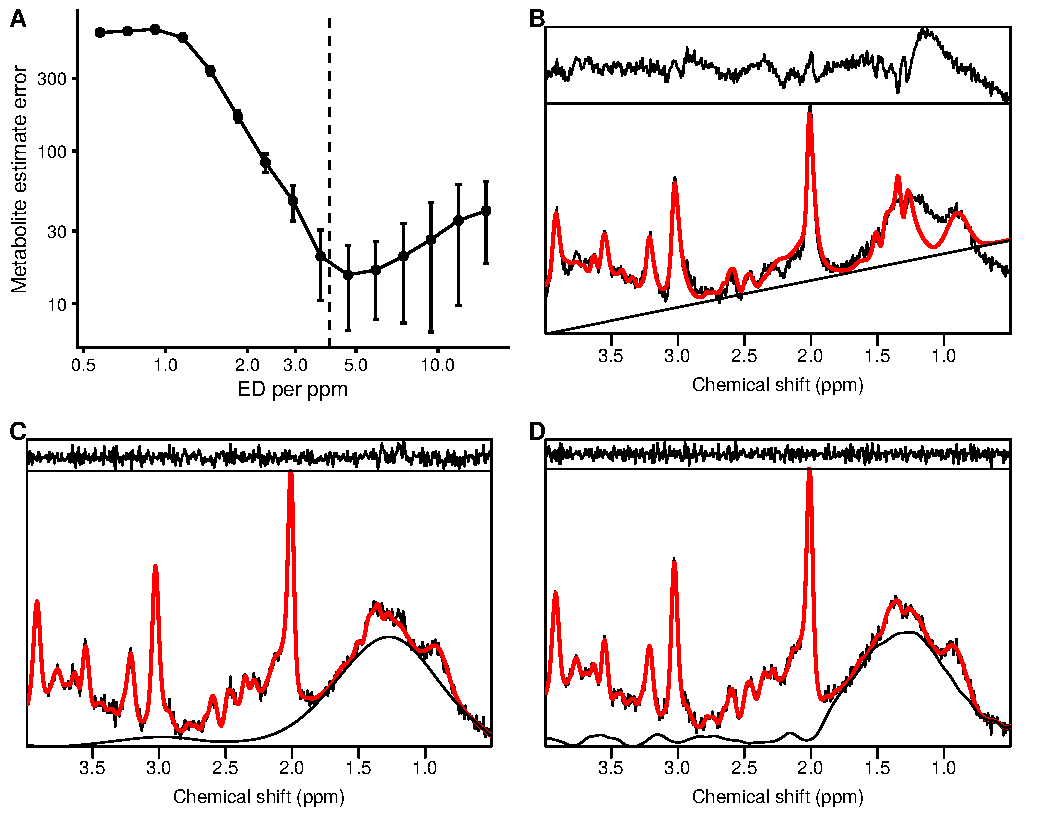
\includegraphics[width=0.8\textwidth]{fig4}
    \caption{ABfit analysis results for simulated data with broad baseline distortion at 1.3 ppm. A) metabolite estimate error of ABfit, with the automatically determined level of baseline flexibility shown as a dashed vertical line. ABfit results with baseline flexibility of B) 0.5, C) 4.1 and D) 15.0 ED per ppm.}
    \label{broad_bl}
  \end{center}
\end{figure}

The baseline distortion was removed for the second simulation study to test the ABfit approach for ideal spectra where the molecular basis alone is sufficient for accurate analysis. The error plot is shown in Figure \ref{flat_bl}, illustrating the absence of bias due to baseline underfitting. A compromise between bias and variance is unnecessary in the ideal case, as the correctly determined baseline flexibility has the lowest error and variability.

\begin{figure}
  \begin{center}
    \includegraphics[width=0.8\textwidth]{fig5}
    \caption{ABfit analysis results for simulated data without baseline distortion. A) metabolite estimate error of ABfit, with the automatically determined level of baseline flexibility shown as a dashed vertical line. ABfit results with baseline flexibility of B) 0.5, C) 4.5 and D) 15.0 ED per ppm.}
    \label{flat_bl}
  \end{center}
\end{figure}

In the third simulation test the amplitude of the broad distortion at 1.3 ppm was doubled compared to the first. A reasonable estimate of the optimal baseline flexibility is found using the ABfit method (Figure \ref{big_broad_bl}A) with comparable levels of accuracy relative to the reduced amplitude baseline distortion (Figure \ref{broad_bl}A).

\begin{figure}
  \begin{center}
    \includegraphics[width=0.8\textwidth]{fig6}
    \caption{ABfit analysis results for simulated data with broad baseline distortion at 1.3 ppm and twice the amplitude compared to Figure \ref{broad_bl}. A) metabolite estimate error of ABfit, with the automatically determined level of baseline flexibility shown as a dashed vertical line. ABfit results with baseline flexibility of B) 0.5, C) 5.1 and D) 15.0 ED per ppm.}
    \label{big_broad_bl}
  \end{center}
\end{figure}

In the fourth simulation test a set of independent broad lipid and macromolecular signals in the basis were used to model the experimentally derived macromolecular profile. Figure \ref{sim_lip_mm_basis}A shows the lowest mean errors are obtained at higher levels of baseline flexibility (part D) --- indicating a stronger bias at lower level of flexibility (parts B, C) compared to the previous simulations. This is likely explained by inadequate modeling of the broad macromolecular components around 3.8 ppm since these are not present in the commonly used individual macromolecular and lipid basis (Supporting Information Table S2).

\begin{figure}
  \begin{center}
    \includegraphics[width=0.8\textwidth]{fig7}
    \caption{ABfit analysis results for simulated data without baseline distortion, but with the true macromolecular basis signal replaced with individually simulated lipid and macromolecular signals. A) metabolite estimate error of ABfit, with the automatically determined level of baseline flexibility shown as a dashed vertical line. ABfit results with baseline flexibility of B) 0.5, C) 1.6 and D) 15.0 ED per ppm.}
    \label{sim_lip_mm_basis}
  \end{center}
\end{figure}

In the final simulation test, the first test was repeated with broader metabolite signals to evaluate the efficacy of the automated baseline determination for poorly shimmed data. Errors are larger compared to the first test, due to the reduction in SNR and spectral resolution, however a reasonable estimate of the optimal baseline flexibility of approximately 4 ED per ppm is found (Figure \ref{broad_bl_bad_shim}A).

\begin{figure}
  \begin{center}
    \includegraphics[width=0.8\textwidth]{fig8.eps}
    \caption{ABfit analysis results for simulated data with broad baseline distortion at 1.3 ppm and metabolite FWHM of 0.1 ppm. A) metabolite estimate error of ABfit, with the automatically determined level of baseline flexibility shown as a dashed vertical line. ABfit results with baseline flexibility of B) 0.5, C) 4.1 and D) 15.0 ED per ppm.}
    \label{broad_bl_bad_shim}
  \end{center}
\end{figure}

\subsection{Experimental}
The results of ABfit applied to experimentally acquired 2D MRSI data are shown in Figure \ref{mrsi_res}. A strong correlation between metabolite levels and the underlying tissue contribution is visually apparent from part A, with an increased tNAA / tCr ratio in white matter compared to gray matter (tNAA = NAA + NAAG, tCr = PCr + Cr, tCho = GPC + PC, Glx = Glu + Gln). A linear regression of select metabolite ratios with the gray matter fraction is plotted in Figure \ref{mrsi_res} parts B, C and D, with strong correlations observed --- in good agreement with high field observations \cite{Nassirpour2018, Hangel2018}. The mean full-width at half maximum resolution across the voxels analyzed was 0.032 ppm, measured from the tNAA resonance. The mean SNR was 85, with the noise region defined as the real valued data points between -0.5 and -2.5 ppm.

Two example fits from one of the voxels in the MRSI data set are shown Figure \ref{lineshape_res}. In part A, the ABfit method is applied as described previously, and in part B the lineshape asymmetry parameter ($a_{g}$) is heavily constrained to enforce a symmetric lineshape model. A smaller fit residual in the tNAA spectral region is found for the asymmetric lineshape model, justifying the minor increase in modeling complexity associated with an additional fit parameter.

\begin{figure}
  \begin{center}
    \includegraphics[width=0.8\textwidth]{fig9}
    \caption{ABfit results from a 2D MRSI semi-LASER acquisition. A) Orthogonal T1 MRI slices intersecting the analysis region --- shown as a colored tNAA / tCr metabolite map overlay. Linear regression of key metabolite ratios with the gray matter fraction are shown in parts B, C and D. The line of best fit is plotted in blue with the 95\% confidence region in gray.}
    \label{mrsi_res}
  \end{center}
\end{figure}

\begin{figure}
  \begin{center}
    \includegraphics[width=0.8\textwidth]{fig10}
    \caption{ABfit result plot for a voxel within a 2D MRSI semi-LASER acquisition with an asymmetric lineshape. A) default analysis with an asymmetric lineshape fit model, B) analysis with the lineshape asymmetry parameter ($a_{g}$) restricted to $\pm 0.0001$.}
    \label{lineshape_res}
  \end{center}
\end{figure}


\section{Discussion and Conclusions}
A new algorithm to automatically determine the optimal level of baseline flexibility has been developed and validated using simulated and acquired MRS data. LCModel is currently the most widely used approach for automatically estimating the optimal baseline flexibility, where the optimal penalty parameter ($\alpha_{B}$) is chosen by gradually increasing its value until the boundary of the 50\% confidence region for the fit is achieved --- estimated by comparing successive fits to the first in the series \cite{Provencher1982, Provencher1993}. In contrast to LCModel, the method presented here uses a modification to the AIC to determine the optimal penalty factor --- as part of a four-step fitting procedure. An additional difference is the use of P-splines in ABfit compared to smoothing spline approach \cite{OSullivan1986} used in LCModel.

Sima and Van Huffel proposed the use of the classical generalized cross-validation (GCV) criterion, combined with a golden-section search, to determine the optimal penalty parameter value \cite{Sima2006}. High accuracy was demonstrated for simulated data, however the method was only tested with good starting values for the non-linear fitting parameters, which are not typically available for experimentally acquired MRS. In ABfit, these non-linear parameters are estimated using a simplified initial fit (step 2) and subsequently refined (step 4). More recently, Zhang and Shen showed that a measure of the baseline uncertainty is also a useful criterion to determine baseline smoothness for simulated and experimentally acquired data \cite{Zhang2014}.

ABfit was shown to find a reasonable compromise between bias and variance for the majority of simulation tests. However, in the fourth simulation test, where the macromolecular basis signals were not identical to those in the simulated data, the optimal flexibility was less easily determined. This is likely due to the bias associated with overly rigid baseline being approximately matched with greater fitting instability from an overly flexible baseline. Reduced SNR would likely enhance the fitting instability and therefore a more rigid baseline would be automatically chosen in this case --- resulting in greater bias. This represents a significant challenge for automated baseline selection, as data with poor SNR will have more biased metabolite levels compared to data with high SNR --- a problem previously identified by Near et al \cite{Near2013} using the LCModel package.

Potential solutions to reduce metabolite estimation bias associated with variable data quality include the use of more accurate macromolecular modeling \cite{Birch2017} and opting to use a fixed level of baseline flexibility. Whist the default approach for ABfit is to automatically select the level of baseline flexibility, fitting options are implemented to specify a fixed degree. Each of these approaches has advantages and weaknesses and should be justified depending on the study aims. For example, in functional-MRS a small change in metabolite levels is generally sought, and therefore a less flexible baseline may be preferred --- since any metabolite estimation bias is eliminated when the change is normalized to a well determined signal.

In conclusion, new MRS analysis method with adaptive baseline modeling is presented and validated on simulated and experimentally acquired data. The approach is fully-automated and integrated into a free and open-source software package --- providing a transparent and reproducible platform for future MRS studies \cite{Stikov2019}.

%\section*{ACKNOWLEDGEMENTS}

\bibliography{main}

\clearpage
\listoffigures

\section*{List of Tables for Supporting Information}
Table S1 Metabolite concentrations consistent with levels measured in normal brain tissue. \\
Table S2 Parameters used to generate the individual simulated lipid and macromolecule basis signals. Listed components with the same name were summed to form a composite signal. \\

\end{document}

%%% Local Variables:
%%% ispell-local-dictionary: "american"
%%% End:
